% This is "sig-alternate.tex" V2.1 April 2013
% This file should be compiled with V2.5 of "sig-alternate.cls" May 2012
%
% This example file demonstrates the use of the 'sig-alternate.cls'
% V2.5 LaTeX2e document class file. It is for those submitting
% articles to ACM Conference Proceedings WHO DO NOT WISH TO
% STRICTLY ADHERE TO THE SIGS (PUBS-BOARD-ENDORSED) STYLE.
% The 'sig-alternate.cls' file will produce a similar-looking,
% albeit, 'tighter' paper resulting in, invariably, fewer pages.
%
% ----------------------------------------------------------------------------------------------------------------
% This .tex file (and associated .cls V2.5) produces:
%       1) The Permission Statement
%       2) The Conference (location) Info information
%       3) The Copyright Line with ACM data
%       4) NO page numbers
%
% as against the acm_proc_article-sp.cls file which
% DOES NOT produce 1) thru' 3) above.
%
% Using 'sig-alternate.cls' you have control, however, from within
% the source .tex file, over both the CopyrightYear
% (defaulted to 200X) and the ACM Copyright Data
% (defaulted to X-XXXXX-XX-X/XX/XX).
% e.g.
% \CopyrightYear{2007} will cause 2007 to appear in the copyright line.
% \crdata{0-12345-67-8/90/12} will cause 0-12345-67-8/90/12 to appear in the copyright line.
%
% ---------------------------------------------------------------------------------------------------------------
% This .tex source is an example which *does* use
% the .bib file (from which the .bbl file % is produced).
% REMEMBER HOWEVER: After having produced the .bbl file,
% and prior to final submission, you *NEED* to 'insert'
% your .bbl file into your source .tex file so as to provide
% ONE 'self-contained' source file.
%
% ================= IF YOU HAVE QUESTIONS =======================
% Questions regarding the SIGS styles, SIGS policies and
% procedures, Conferences etc. should be sent to
% Adrienne Griscti (griscti@acm.org)
%
% Technical questions _only_ to
% Gerald Murray (murray@hq.acm.org)
% ===============================================================
%
% For tracking purposes - this is V2.0 - May 2012

\documentclass{sig-alternate-05-2015}
\usepackage{hyperref}
\usepackage{float}

\begin{document}

% Copyright
\setcopyright{acmcopyright}
%\setcopyright{acmlicensed}
%\setcopyright{rightsretained}
%\setcopyright{usgov}
%\setcopyright{usgovmixed}
%\setcopyright{cagov}
%\setcopyright{cagovmixed}




\title{Http client}
\subtitle{[Ugeopgave 1]
\titlenote{}}
%
% You need the command \numberofauthors to handle the 'placement
% and alignment' of the authors beneath the title.
%
% For aesthetic reasons, we recommend 'three authors at a time'
% i.e. three 'name/affiliation blocks' be placed beneath the title.
%
% NOTE: You are NOT restricted in how many 'rows' of
% "name/affiliations" may appear. We just ask that you restrict
% the number of 'columns' to three.
%
% Because of the available 'opening page real-estate'
% we ask you to refrain from putting more than six authors
% (two rows with three columns) beneath the article title.
% More than six makes the first-page appear very cluttered indeed.
%
% Use the \alignauthor commands to handle the names
% and affiliations for an 'aesthetic maximum' of six authors.
% Add names, affiliations, addresses for
% the seventh etc. author(s) as the argument for the
% \additionalauthors command.
% These 'additional authors' will be output/set for you
% without further effort on your part as the last section in
% the body of your article BEFORE References or any Appendices.

\numberofauthors{1} %  in this sample file, there are a *total*
% of EIGHT authors. SIX appear on the 'first-page' (for formatting
% reasons) and the remaining two appear in the \additionalauthors section.
%
\author{
% You can go ahead and credit any number of authors here,
% e.g. one 'row of three' or two rows (consisting of one row of three
% and a second row of one, two or three).
%
% The command \alignauthor (no curly braces needed) should
% precede each author name, affiliation/snail-mail address and
% e-mail address. Additionally, tag each line of
% affiliation/address with \affaddr, and tag the
% e-mail address with \email.
%
% 1st. author
\alignauthor
Mirza Hasanbasic
}
% There's nothing stopping you putting the seventh, eighth, etc.
% author on the opening page (as the 'third row') but we ask,
% for aesthetic reasons that you place these 'additional authors'
% in the \additional authors block, viz.

% Just remember to make sure that the TOTAL number of authors
% is the number that will appear on the first page PLUS the
% number that will appear in the \additionalauthors section.

\maketitle
\begin{abstract}
In this assignment we will be looking at how to implement a simple HTTP client, that will have a subset of the entire HTTP protocol. The HTTP client will still be able to communicate with servers. There will be performance and validation discussion about the HTTP client as well as the limitations and testing of the client.
\end{abstract}


%
% The code below should be generated by the tool at
% http://dl.acm.org/ccs.cfm
% Please copy and paste the code instead of the example below.
%
\begin{CCSXML}
<ccs2012>
 <concept>
  <concept_id>10010520.10010553.10010562</concept_id>
  <concept_desc>Computer systems organization~Embedded systems</concept_desc>
  <concept_significance>500</concept_significance>
 </concept>
 <concept>
  <concept_id>10010520.10010575.10010755</concept_id>
  <concept_desc>Computer systems organization~Redundancy</concept_desc>
  <concept_significance>300</concept_significance>
 </concept>
 <concept>
  <concept_id>10010520.10010553.10010554</concept_id>
  <concept_desc>Computer systems organization~Robotics</concept_desc>
  <concept_significance>100</concept_significance>
 </concept>
 <concept>
  <concept_id>10003033.10003083.10003095</concept_id>
  <concept_desc>Networks~Network reliability</concept_desc>
  <concept_significance>100</concept_significance>
 </concept>
</ccs2012>
\end{CCSXML}

\ccsdesc[500]{Computer systems organization~Embedded systems}
\ccsdesc[300]{Computer systems organization~Redundancy}
\ccsdesc{Computer systems organization~Robotics}
\ccsdesc[100]{Networks~Network reliability}


%
% End generated code
%

%
%  Use this command to print the description
%


% We no longer use \terms command
%\terms{Theory}


\section{The client}
I have written the HTTP client in python and you are able to run in from a terminal. The file should be executable and in order to run it you need to write two arguments where the first is the desired website you wish to send a request to and the second argument is the name the savefile should have. There is a possibility for a third argument, but this has not been implemented yet. The third argumentive would only have been useful to us since it would work like a debug mode where we can print, but due to time constraint we have not done this.

To run the HTTPclient you simply write the following in the console \texttt{./HTTPclient.py 'website' 'filename'} remember that if you download an \texttt{.exe} file, the filename should have an extension to match it.

The libraries I use are myparser, socket and sys in the HTTP client and in my parser I use itertools and unittest. The unittest is a framework I use in myparser to test if I get a correct output

The function that I use to split my url is \texttt{stringToUrl(myurl)}, where the variable name \texttt{myurl} the string I wish to parse.
I start with splitting after \texttt{'//'} and then I check wether the user have given me \texttt{HTTPS} as input. If this is true, then I raise an error and tell the user that \texttt{HTTPS} is not implemented and that they should use \texttt{HTTP} instead.
After this I check the length of my list. I the length is greater than 1 then the user have written \texttt{http://www.example.com} but if the length is 1 then the user have written \texttt{www.example.com} and if this is true, then I add the \texttt{HTTP} for the user and insert both the scheme and netloc into a list.\footnote{The scheme is 'http' where as the netloc is 'www.example.com'}
From this point I check wether the netloc contains \texttt{:} or \texttt{/}. If the netloc has \texttt{:} then it means that there is a port and I split it. After I split it I add \texttt{:} in between the netloc and the port number i.e. I now have [scheme // netloc : port]. If the netloc have any folder then in my list I have [... port/folder/folder2] and then I need to check if this is true. If there are any folders I split again and then I flatten the list, because I end up with a list of lists. In the end of the parser I add a \texttt{/} after the netloc and \texttt{//} before the netloc so the format should be as \texttt{http\_URL = "http:" "//" host [ ":" port ] [ abs\_path [ "?" query ]]}
For now I only need to implement the query part, so input as \-\texttt{en.wikipedia.org/wiki/Uniform\_Resource\_identifier\#Examples} won't work

The HTTP client will check wether you have given a port as part of the connection string or not. If not, then the default port will be 80.
As for now, I are using \texttt{HTTP/1.0} because it was not possible to connect to some sites with \texttt{HTTP/1.1}.
This HTTP client can do redirect if you should get an error code 30x. It will use recursion to find the new location.
If you should be able to get a status code 200, then the client will write to the filename the \texttt{GET} request.

\subsection{Code structure}
I have two files (\texttt{HTTPClient.py} and \texttt{myurlparser.py}). In the \texttt{HTTPClient.py} i have two functions. One is the clientconnect and the second one handle saving to files. In the \texttt{myurlparser.py} i only have an urlparser as function and this function handles the parse of the url

\subsection{Performance and validation}
The performance of the client is fine. I have manually tried to time the download speed, since I have not had time to implement this yet and the download speed matches the speed when I use google chrome with a 5\% in difference.
In short the validation matches, but only if you download an \texttt{.exe} file. See the subsection testing for more in detail description about this.
The client can redirect the user if you should run into this.


\subsection{Client limitations}
For now, our urlparser doesn't handle a query in the link. This is a limitation in the urlparser the I have implemented.
As I explained in the subsection "Performance and validation" our client doesn't handle other files than \texttt{.exe} since we get some random input in the first line of a file if it is a \texttt{.txt}. In the subsection testing I have explained this and given an example.


\subsection{Testing}
For the urlparser I have unittesting to check wether the code is following the format \texttt{http\_URL = "http:" "//" host [ ":" port ] [ abs\_path [ "?" query ]]}. There are no error and the unittest can be found in urlparser60.py and in the appendix I have a picture of the unittest if you do not wish to run it.

The HTTPclient should be able to download a file, this I have tried and after the file is downloaded I have checked the shasum against what it should be.
The way I do this, is in the console where I write \texttt{./HTTPclient 'website' 'filename'}\footnote{\href{https://download.jetbrains.com/python/pycharm-community-2016.1.3.exe.sha256}{The sha256 sum} and the file I download \href{http://download.jetbrains.com/python/pycharm-community-2016.1.3.exe}{The executable}}. I check the checksum manually, so in my console I run \texttt{shasum -a 256 filename} and it matches the checksum.
But this does only work with \texttt{.exe} files. If I try to check against a \texttt{.txt} or \text{.html} file then in the top of the file I get a random input in the file i.e. the file changes. I have not been able to solve this, so for now the HTTPclient will only work with an \texttt{.exe} file. As an example to the \texttt{.txt} file error I get, I have used \href{http://anonscm.debian.org/viewvc/webwml/webwml/english/mirror/Mirrors.masterlist?view=co}{this site}. As you can see the first line is \text{Site: ftp-master.debian.org} but when I send a request with my HTTPclient and download the file my first line will be \text{1f90} or something else and the second line is \texttt{Site: ftp-master.debian.org} as in the link. So for now this HTTPclient only works for \texttt{.exe} files.

%APPENDICES are optional
%\balancecolumns
\appendix
%Appendix A
\section{Headings in Appendices}
As seen in the picture below, the the unittest is running as it should, with no errors
 
\newpage
\begin{figure}[H]
  \centering
  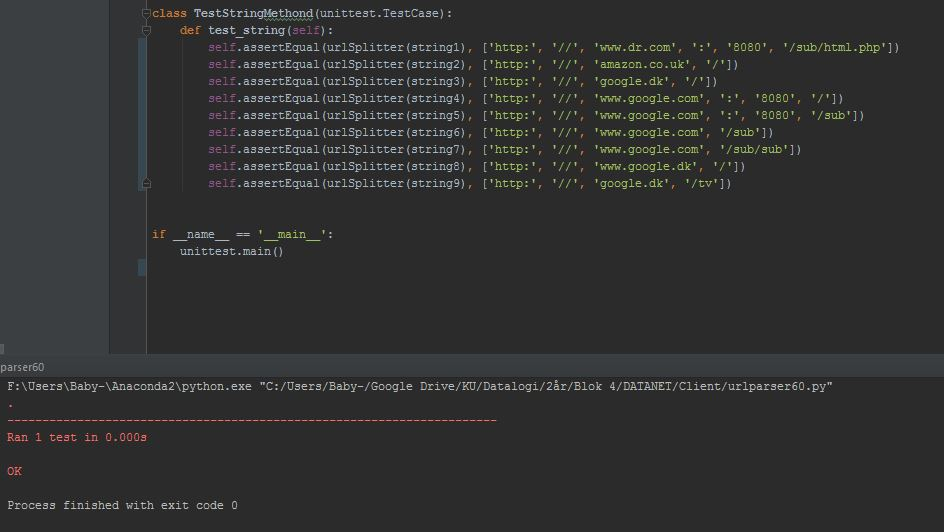
\includegraphics[scale=0.7]{unittestting.jpg}
\end{figure}


%\balancecolumns % GM June 2007
% That's all folks!
\end{document}
